% Options for packages loaded elsewhere
\PassOptionsToPackage{unicode}{hyperref}
\PassOptionsToPackage{hyphens}{url}
\PassOptionsToPackage{dvipsnames,svgnames*,x11names*}{xcolor}
%
\documentclass[
  11pt,
]{article}
\usepackage{amsmath,amssymb}
\usepackage[]{nimbusserif}
\usepackage{ifxetex,ifluatex}
\ifnum 0\ifxetex 1\fi\ifluatex 1\fi=0 % if pdftex
  \usepackage[T1]{fontenc}
  \usepackage[utf8]{inputenc}
  \usepackage{textcomp} % provide euro and other symbols
\else % if luatex or xetex
  \usepackage{unicode-math}
  \defaultfontfeatures{Scale=MatchLowercase}
  \defaultfontfeatures[\rmfamily]{Ligatures=TeX,Scale=1}
\fi
% Use upquote if available, for straight quotes in verbatim environments
\IfFileExists{upquote.sty}{\usepackage{upquote}}{}
\IfFileExists{microtype.sty}{% use microtype if available
  \usepackage[]{microtype}
  \UseMicrotypeSet[protrusion]{basicmath} % disable protrusion for tt fonts
}{}
\makeatletter
\@ifundefined{KOMAClassName}{% if non-KOMA class
  \IfFileExists{parskip.sty}{%
    \usepackage{parskip}
  }{% else
    \setlength{\parindent}{0pt}
    \setlength{\parskip}{6pt plus 2pt minus 1pt}}
}{% if KOMA class
  \KOMAoptions{parskip=half}}
\makeatother
\usepackage{xcolor}
\IfFileExists{xurl.sty}{\usepackage{xurl}}{} % add URL line breaks if available
\IfFileExists{bookmark.sty}{\usepackage{bookmark}}{\usepackage{hyperref}}
\hypersetup{
  pdftitle={JOLTS Overview},
  colorlinks=true,
  linkcolor=blue,
  filecolor=Maroon,
  citecolor=Blue,
  urlcolor=blue,
  pdfcreator={LaTeX via pandoc}}
\urlstyle{same} % disable monospaced font for URLs
\usepackage[width = 140mm, top = 10mm, bottom = 20mm]{geometry}
\usepackage{graphicx}
\makeatletter
\def\maxwidth{\ifdim\Gin@nat@width>\linewidth\linewidth\else\Gin@nat@width\fi}
\def\maxheight{\ifdim\Gin@nat@height>\textheight\textheight\else\Gin@nat@height\fi}
\makeatother
% Scale images if necessary, so that they will not overflow the page
% margins by default, and it is still possible to overwrite the defaults
% using explicit options in \includegraphics[width, height, ...]{}
\setkeys{Gin}{width=\maxwidth,height=\maxheight,keepaspectratio}
% Set default figure placement to htbp
\makeatletter
\def\fps@figure{htbp}
\makeatother
\setlength{\emergencystretch}{3em} % prevent overfull lines
\providecommand{\tightlist}{%
  \setlength{\itemsep}{0pt}\setlength{\parskip}{0pt}}
\setcounter{secnumdepth}{-\maxdimen} % remove section numbering
\ifluatex
  \usepackage{selnolig}  % disable illegal ligatures
\fi
\usepackage[]{natbib}
\bibliographystyle{aea}

\title{JOLTS Overview}
\author{}
\date{\vspace{-2.5em}}

\begin{document}
\maketitle

\hypertarget{introduction}{%
\subsection{Introduction}\label{introduction}}

How well the labor market is performing is a much more complicated
process than simply asking what the current unemployment rate is. While
a lower rate of unemployment is surely an important indicator of the
strength of the labor market, there are many factors that are of equal
importance. But why are labor market conditions so important? Labor
market conditions are prominent in the monetary policy deliberations of
the Federal Reserve's Federal Open Market Committee (FOMC). The
objectives Congress gave the Fed for monetary policy are ``maximum
employment, stable prices, and moderate long-term interest rates.'' It's
natural then that labor market conditions are an integral part of
monetary policy deliberations.

The Job Openings and Labor Turnover Survey (JOLTS) tells us how many job
openings there are each month, how many workers were hired, how many
quit their job, how many were laid off, and how many experienced other
separations (which includes worker deaths).

We review some of the theoretical literature and stylized facts
regarding the labor market in the United States. This document is by no
means a thorough review of all the literature on the subject, but it
does aim to present the leading theories and evidence. For those
unfamiliar with the concepts in time series methodologies, there is a
brief overview of the main methods and guiding principles.

\hypertarget{data}{%
\subsection{Data}\label{data}}

The JOLTS survey design is a stratified random sample of 20,700 nonfarm
business and government establishments. The sample is stratified by
ownership, region, industry sector, and establishment size class. The
establishments are drawn from a universe of over 9.4 million
establishments compiled by the Quarterly Census of Employment and Wages
(QCEW) program which includes all employers subject to state
unemployment insurance laws and federal agencies subject to the
Unemployment Compensation for Federal Employees program.

Employment estimates are benchmarked, or ratio adjusted, monthly to the
strike-adjusted employment estimates of the Current Employment
Statistics (CES) survey. A ratio of CES to JOLTS employment is used to
adjust the levels for all other JOLTS data elements.

The JOLTS estimates also are affected by nonsampling error. Nonsampling
error can occur for many reasons including: the failure to include a
segment of the population; the inability to obtain data from all units
in the sample; the inability or unwillingness of respondents to provide
data on a timely basis; mistakes made by respondents; errors made in the
collection or processing of the data; and errors from the employment
benchmark data used in estimation.\footnote{Nonsampling error occurs
  when a sample is surveyed rather than the entire population. Which
  means that there is a chance that the sample estimates may differ from
  the true population values they represent. The difference, or sampling
  error, varies depending on the particular sample selected. This
  variability is measured by the standard error of the estimate. BLS
  analysis is generally conducted at the 90-percent level of confidence.
  That means that there is a 90-percent chance, or level of confidence,
  that an estimate based on a sample will differ by no more than 1.6
  standard errors from the true population value because of sampling
  error. Sampling error estimates are available at the BLS'
  \href{https://www.bls.gov/jlt/jolts_median_standard_errors.htm}{website}}

\hypertarget{background}{%
\subsection{Background}\label{background}}

As the United States reels from the COVID-19 pandemic's catastrophic
economic damage, the tight labor markets from early 2020 seem like a
distant memory. Before the COVID-19 pandemic, the U.S. labor market had
been steadily improving for years: the unemployment rate was falling for
nearly a decade to rates not seen since the late 1960s, and witnessed
the longest streak of private sector job creation on record. Given these
impressive headline statistics, it may come as a surprise that
unemployed workers had slightly more trouble finding a job than they did
at the peak of the last business cycle (in 2006) and have a much lower
probability of finding a job than in 2000.

What makes the COVID-19 recession unique is the nature of the initial
shock. While past recessions have been primarily caused by economic or
financial shocks, the adverse shock to the labor market in 2020 was
triggered by a novel virus that forced millions of employees into
temporary unemployment by the second quarter of 2020. The record-level
rise in temporary unemployment contrasts starkly with past recessions
that typically start with an increase in permanent layoffs
\citep{elsby10}.

The path of job vacancies has also been unusual: while vacancies fell
throughout the first half of 2020, the drop was much less pronounced
than is typical in most recessions. In fact, vacancies at their lowest
level were equal to the level that prevailed in 2015, a time typically
considered to be a tight labor market. Thus, while the Beveridge curve
-- the negative relationship between vacancies and unemployment --
typically ``loops around'' during and after a recession, in the early
months of the COVID-19 recession, the increase in the unemployment rate
was much larger than the corresponding drop in job vacancies.

\begin{center}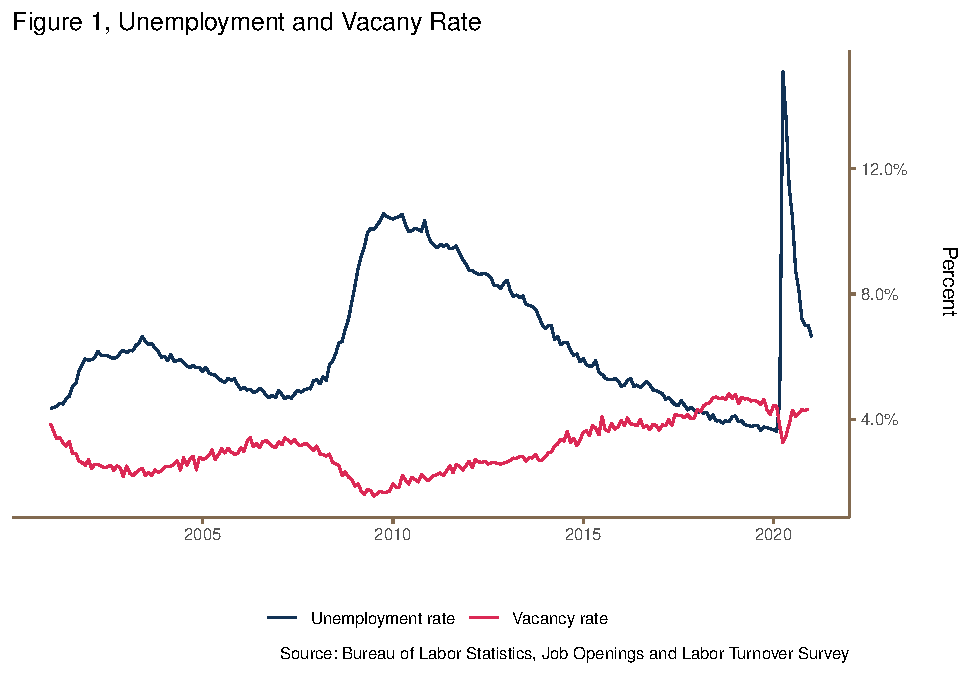
\includegraphics{JOLTS_files/figure-latex/unnamed-chunk-5-1} \end{center}

The difference is that the prior recessions were caused by ``demand''
shocks; the current recession is fundamentally a ``supply'' shock. The
current recession tore away the facade of the recovery from the Great
Recession, exposing the core issues facing the U.S. economy that really
had been accumulating over the last three decades: namely increasing
inequality and decreasing dynamism in the labor market.

\begin{center}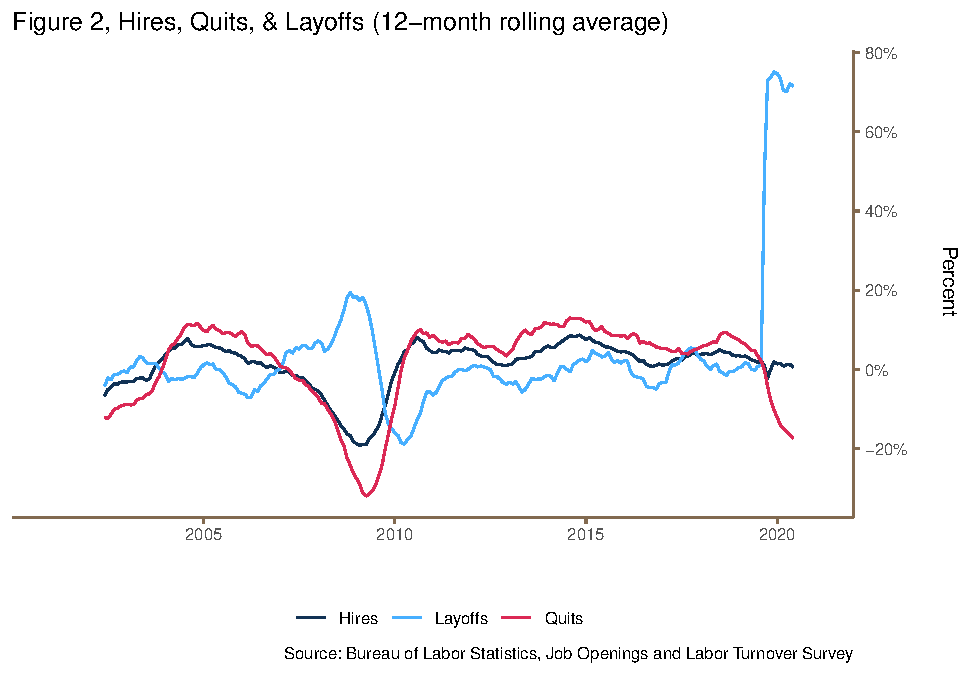
\includegraphics{JOLTS_files/figure-latex/unnamed-chunk-6-1} \end{center}

During the late 1990s, roughly 30--35 percent of the unemployed found a
job within a month; in 2006 according to estimates by \cite{Fallick04},
just prior to the Great Recession, the rate peaked at an annual average
of 28.3. Over the course of the recession and for many years afterwards,
the probability that an unemployed worker found a job would remain
relatively low, with an annual average of 17.0 percent in 2010. Only
over the last two years has the probability risen back into the 25--30
percent range, and it stood at 27.7 percent in 2018. These trends are
depicted in Figure 3.

\begin{center}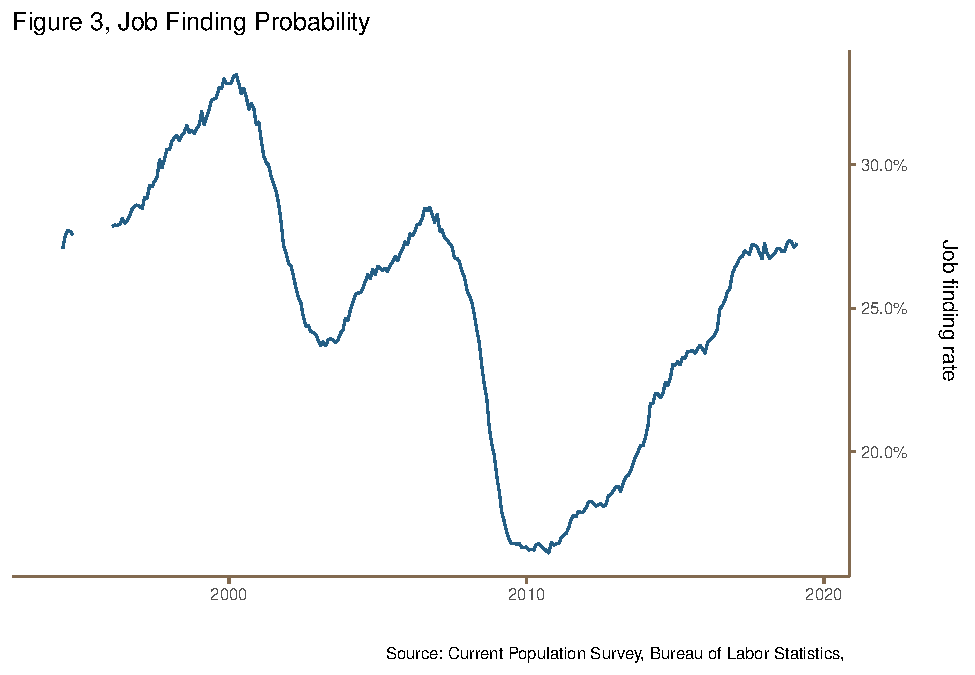
\includegraphics{JOLTS_files/figure-latex/unnamed-chunk-7-1} \end{center}

Like the vacancy rate, the job-finding rate moves inversely with the
unemployment rate, though the correlation is not perfect. As the
unemployment rate initially began to decline at the beginning of the
recovery from the Great Recession, the job-finding probability did not
increase as quickly. The sustained depression in job-finding was a
primary factor that prolonged high U.S. unemployment; today, a
relatively high job-finding rate helps keep unemployment low.

Prior to the pandemic induced the job-finding rate was still slightly
lower than in 2006 despite an unemployment rate nearly a percentage
point lower. To better understand how the job-finding rate has changed
over time and why it remains somewhat lower than one might expect, we
look at how the probability of finding a job changes with length of
unemployment.

The decline in the job finding rate implies that the unemployed
increasingly spend longer spells of unemployment than previously.
Indeed, as Figure 4 shows, the distribution of unemployment duration.
Elevated unemployment durations reflect an economy with fewer startups,
less job reallocation, and diminished dynamism more generally. Both
job-finding and job-losing have declined over time, leaving the
unemployment rate roughly at its 2000 level despite a
4.6-percentage-point decline in job-finding. (Elevated unemployment
durations may also have other causes, for example the increase in wage
inequality, which leads job searchers to hold out for the highest-paid
opportunities.)

\begin{center}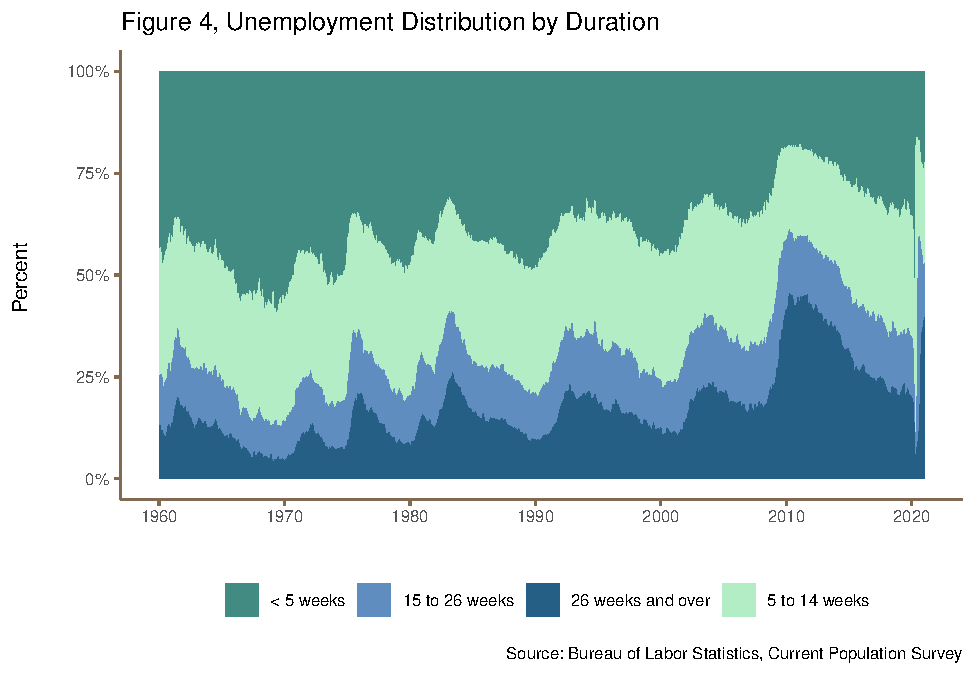
\includegraphics{JOLTS_files/figure-latex/unnamed-chunk-8-1} \end{center}

One of the most direct measures of declining labor market dynamism is
the rate of job creation. Job creation combines the employment gains at
new and growing establishments. While there has been some cyclical
fluctuation, job creation as a share of employment has been on a long
downward trend since the early 1990s \citep{davis14}. We can visualize
the outcome of this declining trend in the employment growth rate of
Figure 5. Up until the early 1990s, employment growth in the United
States rebounded from recessions, but this pattern has since erroded at
the close of the 1990s.

\begin{center}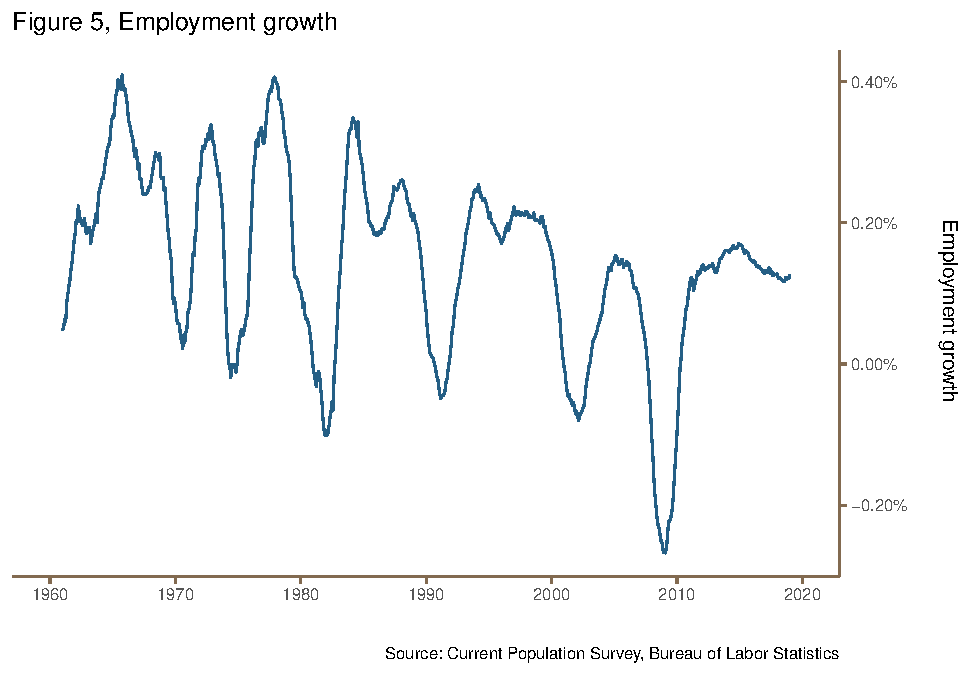
\includegraphics{JOLTS_files/figure-latex/unnamed-chunk-9-1} \end{center}

At the same time, workers are increasingly less likely to switch jobs.
This decline matters for wage growth. First, at least one-third of all
hires are made among those already employed, suggesting that job
switching is a integral part of how workers' careers evolve; and second,
part of the decline in hiring comes from the decline in job switching.
Indeed, more than 40 percent of the decline in hires and separations can
be ascribed to declining job-to-job transitions \citep{Hyatt13}. As
workers generally receive a raise when they transition directly from one
job to another, declining job switching has put downward pressure on
wage growth.

These are not the only statistical measures showing declining
flexibility in the U.S. labor market. There have been substantial
declines in dynamism---sometimes referred to as labor market
fluidity---across a variety of related measures. When job creation, job
destruction, job switching, interstate migration, and other indicators
of fluidity are combined, \cite{Molloy16} find that labor market
fluidity has been on a downward trend since at least the 1980s, and has
fallen by 10 to 15 percent since the 1990s.

Estimation of the job finding probability comes from a line of research
in the so-called ``Search-Theoretic'' approach to unemployment and
duration analysis \citep{Pissarides2000}. Duration analysis has its
origins in survival analysis, a branch of statistics for analyzing the
expected duration of time until one or more events happen, such as death
in biological organisms and failure in mechanical systems
\citep{Lanc90}. It involves the modeling of time to event data; in our
context, finding a job or becoming unemployed is considered an
``event.'' Since in the social sciences, we are interested in any
situation where an individual or family, or firm, and so on begins in an
initial state and is either observed to exit the state or is censored.

Duration analysis typically begins by specifying a population
distribution for the duration, usually conditional on some explanatory
variables observed at the beginning of the duration. For example, for
the population of people who became unemployed during a particular
period, we might observe education levels, experience, marital
status-all measured when the person becomes unemployed-wage on prior
job, and a measure of unemployment benefits. Then we specify a
distribution for the unemployment duration conditional on the
explanatory variables. Any reasonable distribution reflects the fact
that an unemployment duration is non-negative. Once a complete
conditional distribution has been specified, maximum likelihood methods
are used to estimate the expected duration.

The hazard function allows us to approximate the probability of exiting
the initial state within a short interval, conditional on having
survived up to the starting time of the interval. In econometric
applications, hazard functions are usually conditional on some
covariates.

The survival function \(S(t)\), is the probability that a subject
survives or in this case endures longer than time \(t\). If time is
continuous with a cumulative distribution function (cdf) \(F(t)\) then
the survival function is \begin{equation}
\begin{gathered}
S(t) = \mathrm{P}(\{T > t\}) = \int\limits_{t}^{\infty} f(u)\, du \\[8pt]
= 1 - F(t)
\end{gathered}
\end{equation} and this is the probability of ``surviving'' past time
\(t\). The density of \(T\) can be denoted \[
f(t) = \frac{\partial F}{\partial t}(t)
\] The probability that a person who has occupied a state for time \(t\)
leaves it in some short interval \(h\) after \(t\) is given by, \[
\mathrm{P}(t \leq T < t + h \; | \; T \geq t)
\] The hazard or ``exit'' function is
then,\footnote{In engineering this function is called the "failure rate".}
\begin{equation}
\lambda(t) = \lim_{h \;|\, 0} \frac{\mathrm{P}(t \leq T < t + h \; | \; T \geq t)}{h}
\end{equation}

For each \(t\), \(\lambda(t)\) is the instantaneous rate of leaving per
unit of
time.\footnote{This notation follows \cite{Wool01}. \cite{Lanc90} uses $\theta$ in place of the more commonly used $\lambda$ for the hazard rate and uses $dt$ for $h$. Nevertheless, the derivation and formulation in both are equivalent.}

A rough interpretation of \(\lambda(t)\) is that it presents the
probability of exit from a state in the short interval \(h\) after
\(t\), conditional on the state being occupied at \(t\). Put another
way, the hazard function gives the probability that a person unemployed
for 10 weeks (\(\lambda(10)\)) will find employment (exit unemployment),
whereas the unconditional probability provides the chances that a person
will get job at the tenth week of unemployment. That is \(\lambda(10)\)
gives the probability that a person will find a job between weeks 10 and
11, conditional on being unemployed through week 10.

We can express the hazard function and the unconditional probability of
exit in terms of the distribution and the probability density function
(pdf) of \(T\), which is considered to be a continuous random variable.
By the law of conditional probability,

\begin{equation}
\begin{gathered}
\frac{\mathrm{P}(t \leq T < t + h \; | \; T \geq t)}{\mathrm{P}(T \geq t)} \\[8pt]
= \frac{F(t + h) - F(t)}{1 - F(t)}
\end{gathered}
\end{equation}

When the cdf is differentiable, we can take the limit of the right-hand
side, divided by \(h\), as \(h\) approaches zero:

\begin{equation}
\begin{gathered}
\lambda(t) = \lim_{h \to 0} \frac{F(t + h) - F(t)}{h}\cdot \frac{1}{1 - F(t)} \\[8pt]
= \frac{\partial F}{\partial t}F(t) \cdot \frac{1}{1 - F(t)} \\[8pt]
= \frac{f(t)}{1 - F(t)} \\[8pt]
= \frac{f(t)}{S(t)}
\end{gathered}
\end{equation}

Because the first derivative of \(S(t)\) is \(-f(t)\) we can also
express the hazard function as

\begin{equation}
\lambda(t) = - \frac{\partial \ln S(t)}{\partial t}
\end{equation}

Equation (5) is a differential equation in \(t\), whose solution,
subject to the initial condition \(F(0) = 0\) we arrive through
integration

\begin{equation}
F(t) = 1 - \exp\left[\int\limits_{0}^{t}\,\lambda(s)\,ds \right], \quad t \geq 0
\end{equation}

differentiation of equation (6) gives the density of \(T\) as

\begin{equation}
f(t) = \lambda(t)\exp\left[\int\limits_{0}^{t}\,\lambda(s)\,ds \right],
\end{equation}

The shape of the hazard function is important in many empirical aspects
and in the simplest case it is constant \(\lambda(t) = \lambda\). This
function means that the process driving \(T\) is memoryless: the
probability of exit in the next interval does not depend on how much
time has been spent in the initial state. A constant hazard implies

\[
F(t) = 1 - e^{-\lambda t}
\]

When the hazard function is not constant, the process exhibits duration
dependence \citep{Lanc90, vdb96}. Assuming that \(\lambda(t)\) is
differentiable, there is positive duration dependence at time \(t\) if
\(\partial\lambda(t)/\partial t > 0\), then the process exhibits
positive duration dependence. Positive duration dependence means simply
that the probability of exiting the initial state increases the longer
one is in the initial state. If the derivative is negative, however,
then there is negative duration dependence; longer spells in the initial
decreases the probability of exit.

\cite{elsby09b} argue that movements in the job finding probability
accounted for about 65 percent of unemployment fluctuations prior to the
last two recessions, and more in 1990--1991 and 2001. \cite{fujita09}
claim a more substantial role for the hazard rate to unemployment
(separation rate) but still find that the job finding probability
accounts for at least half of the fluctuations in unemployment.

Following the approach of \cite{Shimer12}, we can roughly approximate
the hazard rate (job finding probability) as

\begin{equation}
F_{t} = 1 - \frac{u_{t} - s_{t}}{u_{t-1}}
\end{equation}

which expresses the monthly outflow finding probability as a function of
the total unemployment level \(u_{t}\) at time \(t\) and short term
unemployment \(s_{t}\), defined as those unemployed for less than five
weeks.

Shimer's method extended by \cite{elsby13} shows that the monthly
outflow hazard rate, \(f(t)\) can be transformed from (8) into a
continuous-time outflow hazard as,

\begin{equation}
f_{t} = - \ln(1 - F_{t})
\end{equation}

Calculating this measure from BLS aggregate unemployment duration flows
allows us to look at a longer view of the job finding probability in
Figure 6.

\begin{center}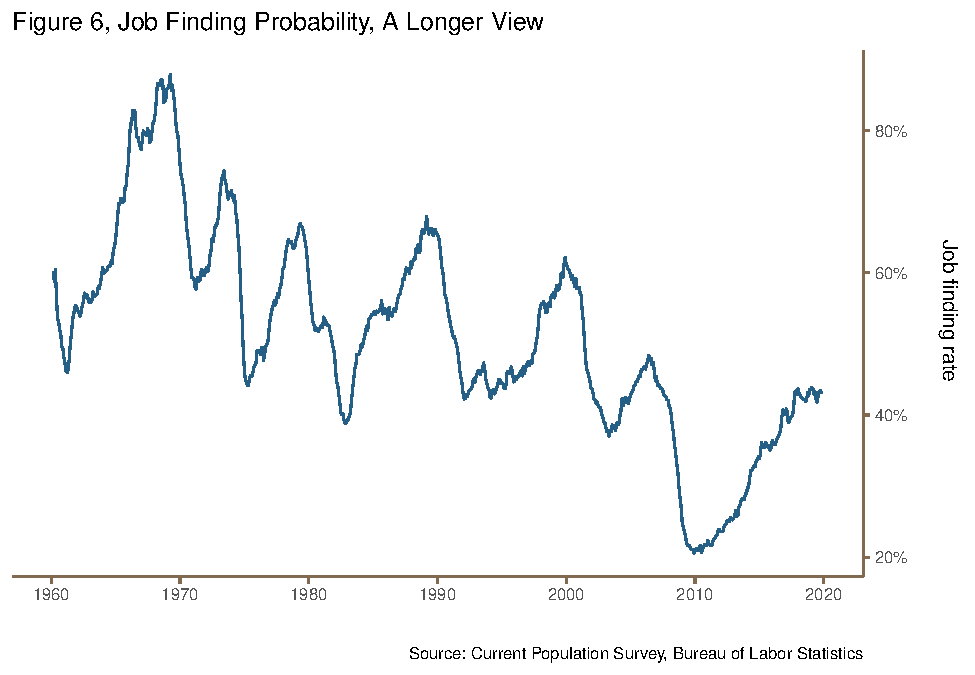
\includegraphics{JOLTS_files/figure-latex/unnamed-chunk-10-1} \end{center}

\cite{Shimer12} argues that fluctuations in the unemployment rate are
mostly explained by fluctuations in job finding rates or transitions out
of unemployment (``Outs'') rather than by fluctuations in job separation
rates or transition into unemployment (``Ins''). This implies that the
unemployment rate fluctuates over the business cycle not because workers
lose their jobs but because workers have a hard time finding a job.

The declining job finding probability is worrying for a number of
reasons. A large literature documents that a particular type of
long-term unemployment - those resulting from job losses during mass
layoffs - leave a very persistent ``scarring'' effect on the future
earnings of displaced
workers.\footnote{A displaced worker is someone who lost their job through no fault of their own, typically this means they were "laid off."}
Future earnings of people who experienced prolonged spells of
unemployment decline by as much as 20 percent \cite{davis10}. A more
recent study by \cite{Guvenen17} finds that the loss is potentially
larger at around 35-40 percent. Furthermore, due to negative duration
dependence, the probability of receiving a callback for an interview
significantly decreases with the length of a worker's unemployment
spell, with the majority of this decline occurring during the first
eight months \cite{kroft13}. In short, what economists call ``negative
duration dependence'' undermines the functioning of the labor market and
generates large social costs.

\begin{center}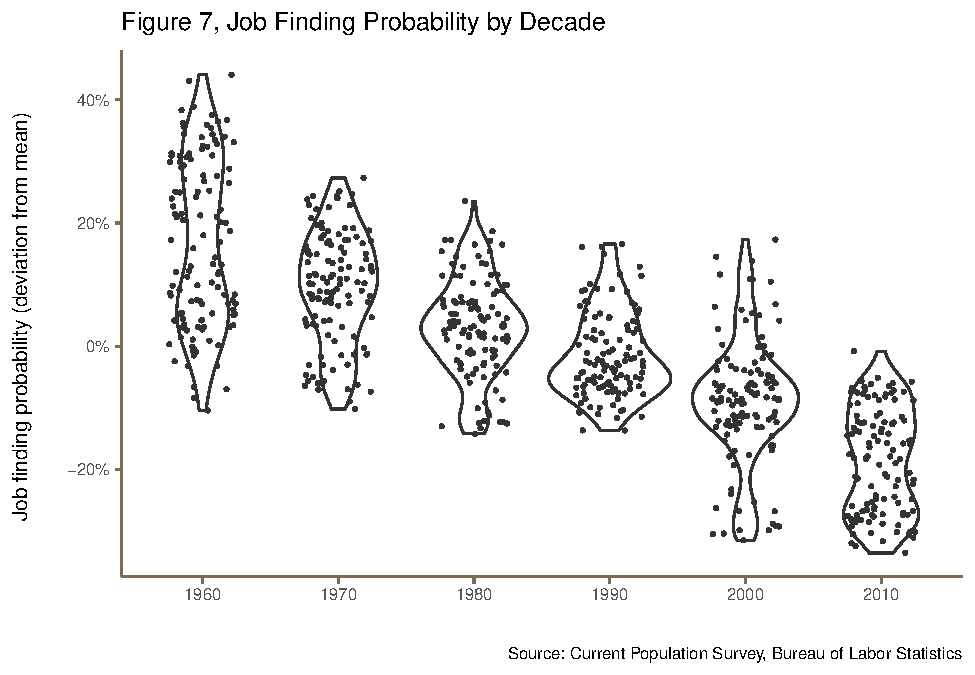
\includegraphics{JOLTS_files/figure-latex/unnamed-chunk-11-1} \end{center}

The unusual nature of the COVID-19 recession makes it difficult to draw
on experiences from past recessions to project how the labor market will
evolve in the months ahead. For example, during the Great Recession, the
initial wave of layoffs was subsequently followed by a prolonged period
of lower job finding rates \citep{elsby09}. This led to a significant
increase in the long-term unemployment share, which in turn prolonged
the recession through negative duration dependence \citep{krueger14}.
Currently available data suggest that the dynamics of the COVID-19
recession may play out quite differently. Looking more closely at the
last two decades in Figure 8 we see that job finding rates have not
decreased as substantially as they did in the Great Recession.

The pandemic is an urgent reminder of what long-term labor trends have
been illustrating for years: low-wage workers need better pathways into
decent jobs, and from shrinking occupations to the jobs of tomorrow.
Policymakers face a dual imperative: to facilitate safe reemployment as
soon as possible, even as COVID-19 continues to surge in many parts of
the country, while also helping low-wage workers on the journey to jobs
with dignity, stability, and a fair shot at economic mobility. While the
risk of mass unemployment has already spurred large public expenditures,
more funding and efforts are needed to ensure opportunity reaches those
who need it the most.

\hypertarget{methods}{%
\subsection{Methods}\label{methods}}

We produce forecasts using a collection of traditional and
non-traditional time series methods. This section provides a general
overview of the methods used, their benefits, and their limitations. It
cannot be emphasized enough that, no matter the strength of a model, it
remains exactly that: a model. As such, all statistical models are
``wrong.'' No matter the method used, any model is an attempt to
reproduce (``model'') the true data generating process of a data series.

\hypertarget{theorectical-background}{%
\subsection{Theorectical Background}\label{theorectical-background}}

For many familiar with the methodology of time series forecasting, this
section presents a brief recapitulation of basic concepts which can be
found in any standard textbook such as \cite{MJK} or \cite{brockwell02}.
For a more advanced treatment, one should see \cite{hamilton94} or
\cite{brockwell06}.

Time series analysis is the procedure of using known data values to fit
a time series with a suitable model and estimation of the corresponding
parameters. It comprises methods that attempt to understand the nature
of the time series.

A major assumption that often provides relief in modeling efforts is the
linearity assumption. A linear filter, for example, is a linear
operation from one time series \(x_{t}\) to another time series
\(y_{t}\).

\begin{equation}
E[y_{t}] = L(x_{t}) = A(L^{i})\epsilon_{t} = \left(\sum\limits_{-\infty}^{\infty} \psi_{i}L^{i}\right)\epsilon_{t} = \mu + \sum\limits_{-\infty}^{\infty}\psi_{i}\epsilon_{t-i},
\end{equation}

where \(\epsilon \sim \mathcal{N}(0, \sigma^{2})\) and \(L^{i}\) is the
Lag or Backshift Operator defined as,

\[
L^{i}x_{t} = x_{t-i} \; \forall \, i \in \mathbb{N}
\]

the linear filter can be seen as a process that converts the input,
\(x_{t}\), into an output, \(y_{t}\) with a conversion process that
involves all (present, past, and future) values of the input in the form
of a summation with different ``weights'', \(\psi_{i}\), on each
observation \(x_{i}\). Specifically, \(y_{t}\) can be expressed as

\[
y_{t} = \mu + \sum\limits_{i= o}^{\infty}\psi_{i}\epsilon_{t-i}
\]

where the weights are conventionally some form of moving average \(M\).
A moving average \(M\) of span \(N\) assigns weights \(\frac{1}{N}\) to
the most recent observations such that the estimate can be written as

\[
M_{t} = \frac{1}{N} \sum\limits_{t = T - N - 1}^{N} y_{t}
\]

The covariance between \(y_{t}\) and its value at another point in time
\(y_{t + k}\) is called the auto-covariance at lag \(k\), and is defined
by

\[
\gamma_{k} = \mathrm{Cov}(y_{t}, y_{t+k}) = E\left[(y_{t} - \mu)(y_{t+k} - \mu)\right]
\]

the autocovariance of the series at lag \(k = 0\) is simply the variance
of the time series. The autocorrelation coefficient at \(k\) is then

\begin{gather*}
\rho_{k} = \frac{E[(y_{t} - \mu)(y_{t+k} -\mu)]}{\sqrt{E[(y_{t} - \mu)^{2}]E[(y_{t+k} - \mu)^{2}]}} \\[8pt]
= \frac{\mathrm{Cov}(y_{t}, y_{t+k})}{\mathrm{Var}(y_{t})}\\[8pt]
= \frac{\gamma_{k}}{\gamma_{0}}
\end{gather*}

The collection of these values \(\rho_{k}\) is called the
autocorrelation function. For a finite time series, it is necessary to
estimate the autocovariance and autocorrelation functions. A usual
estimate of the autorcovariance function is

\[
c_{k} = \hat{\gamma_{k}} = \frac{1}{T} \sum\limits_{t = 1}^{T-k}(y_{t} -\bar{y})(y_{t+k} - \bar{y}), \quad k = 1, 2, 3,\, \ldots,\, K
\] and the autocorrelation function is estimated by the sample
autocorrelation function (sample ACF) \[
r_{k} = \hat{\rho_{k}} = \frac{c_{k}}{c_{o}}
\] The stationarity of a time series is related to its statistical
properties in time. That is, in the more strict sense, a stationary time
series exhibits similar ``statistical behavior'' in time and this is
often characterized as a constant probability distribution in time.
However, it is usually satisfactory to consider the first two moments of
the time series and define stationarity (or weak stationarity) as
follows: (1) the expected value of the time series does not depend on
time and (2) the autocovariance function defined as
\(\mathrm{Cov}(y_{t}, y_{t+k})\) for any lag \(k\) is only a function of
\(k\) and not time: that is, \(y(k) = \mathrm{Cov}(y_{t}, y_{t+k})\).
Weak stationarity, then, implies that the mean of the series does not
change with time \(t\) and that the autocovariance function,
\(\gamma(k, t)\), depends on \(k\) and \(t\) only through their
difference \(k - t\).

For a time-invariant and stable linear filter a stationary input time
series \(y(t)\) can be written more succinctly as,

\begin{gather*}
y(t) = \mu + \sum\limits_{i= 0}^{\infty}\psi_{i}\epsilon_{t} \\[8pt]
\mu + \sum\limits_{i=0}^{\infty}\psi_{i}L^{i}\epsilon_{t} \\[8pt]
\mu + \Psi(L)\epsilon_{t}
\end{gather*}

where \[
  \Psi(L)\epsilon_{t} = \sum\limits_{i=0}^{\infty}\psi_{i}L^{i}
  \]\\
The infinite moving average model has a covariance function in the form,

\[
\mathrm{Cov}(y_{t}, y_{t+k}) = \gamma_{y}(k, t) = \sum\limits_{i = -\infty}^{\infty}\sum\limits_{j = - \infty}^{\infty}\psi_{i}\psi_{j}\gamma_{x}(i - j + k)
\]

The autocovariance function of \(y_{t}\) is then,

\begin{gather*}
\gamma_{y}(k, t) = \sum\limits_{i = o}^{\infty}\sum^{\infty}\limits_{j = 0} \psi_{i}\psi_{j}\gamma_{\epsilon}(i-j+k) \\[8pt]
= \sigma^{2}\sum\limits_{i = 0}^{\infty}\psi_{i}\psi_{i + k}
\end{gather*}

This representation comes from a theorem by Wold and which essentially
states that any nondeterministic weakly stationary time series \(y_{t}\)
can be represented as in the above manner. A more intuitive
interpretation of this theorem is that a stationary time series can be
seen as the weighted sum of the present and past random
``disturbances.''

Although very powerful in providing a general representation of any
stationary time series, the infinite moving average model given in is
not very useful in practice except for certain special cases.

In finite order moving average or MA models, weights that are not set to
0 are represented by the Greek letter \(\theta\) with a minus sign in
front.

\begin{gather*}
y_{t} = \mu + \left(1 - \sum\limits_{i=1}^{q}\theta_{i}L^{i} \right)\epsilon_{i}\\[8pt]
= \mu + \Theta(L)\epsilon_{t}
\end{gather*}

where
\(\Theta(L)\epsilon_{t} = 1 - \sum\limits_{i=1}^{q}\theta_{i}L^{i}\)

An interpretation of the finite order MA processes is that at any given
time, of the infinitely many past disturbances, only a finite number of
the disturbances ``contribute'' to the current value of the time series
and that the time window of the contributors ``moves'' in time, making
the ``oldest'' disturbance obsolete for the next observation. It is
indeed not too far fetched to think that some processes might have these
intrinsic dynamics. However, for some others, we may be required to
consider the ``lingering'' contributions of the disturbances that
happened back in the past. This will of course bring us back to square
one in terms of our efforts in estimating infinitely many weights.
Another solution to this problem is through autoregressive models in
which the infinitely many weights are assumed to follow a distinct
pattern and can be successfully represented with only a handful of
parameters. We shall now consider some special cases of autoregressive
processes.

\hypertarget{arma}{%
\subsection{ARMA}\label{arma}}

Autoregressive models are based on the idea that current value of the
series, \(x_{t}\) can be explained as a linear combination of past
values, \(x_{t-1}, x_{t-2}, \ldots, \, x_{t-p}\), together with some
random error \(\epsilon\). In other words, a series \(x_{t}\) is
linearly dependent upon its past values, the degree to which depends on
the lag order \(p\).

Let us first consider again the time series

\begin{gather*}
y(t) = \mu + \sum\limits_{i= 0}^{\infty}\psi_{i}\epsilon_{t} \\[8pt]
\mu + \sum\limits_{i=0}^{\infty}\psi_{i}L^{i}\epsilon_{t} \\[8pt]
\mu + \Psi(L)\epsilon_{t}
\end{gather*}

One approach to modeling this time series is to assume that the
contributions of the disturbances that are way in the past should be
small compared to the more recent disturbances that the process has
experienced. Since the disturbances are independently and identically
distributed random variables, we can simply assume a set of infinitely
many weights in descending magnitudes reflecting the diminishing
magnitudes of contributions of the disturbances in the past.

A simple and yet intuitive set of such weights can be created following
an exponential decay pattern. For that we will set
\(\psi_{i} = \phi^{i}\), where \(\left|\,\phi\,\right| < 1\) to
guarantee the exponential ``decay.'' In this notation, the weights on
the disturbances starting from the current disturbance and going back in
past will be \(1, \phi^{2}, \phi^{3},\, \ldots\)

\begin{gather*}
y_{t} = \mu + \epsilon_{t} + \phi\epsilon_{t-1} + \phi^{2}\epsilon_{t-2} + \cdots\\[8pt]
= \mu + \sum\limits_{i=0}^{\infty}\phi^{i}\epsilon_{t-i}
\\[8pt]
\end{gather*}

We also have

\begin{gather*}
y_{t-1} = \mu + \epsilon_{t-1} + \phi\epsilon_{t-2} + \phi^{2}\epsilon_{t-3} + \cdots \\[8pt]
= \mu + \phi\left(\sum\limits_{i=0}^{\infty}\phi^{i}\epsilon_{t-1-k} + \epsilon_{t}\right)
\end{gather*}

combining these two equations together we can represent an AR(1) model
as a linear process given by

\begin{gather*}
\mu + \sum\limits_{i=0}^{\infty}\phi^{i}\epsilon_{t-i} = \mu + \phi\left(\sum\limits_{i=0}^{\infty}\phi^{i}\epsilon_{t-i} + \epsilon_{t}\right) \\[8pt]
\mu + \epsilon_{t} + \sum\limits_{i=0}^{\infty}\phi^{i}y_{t-i} + \phi\mu \\[8pt]
\mu - \phi\mu + \sum\limits_{i=0}^{\infty}\phi^{i}y_{t-i} + \epsilon_{t} \\[8pt]
\delta + \sum\limits_{i=0}^{\infty}\phi^{i}y_{t- i} + \epsilon_{t}
\end{gather*}

where \(\delta = (1 - \phi)\mu\). A more general way of writing an
autoregressive procress is through operator notation as

\begin{gather*}
\epsilon_{t} = \left(1 - \sum\limits_{i=1}^{i}\phi_{i}L^{i} \right)y_{t} \\[8pt]
 = \Phi(L)y_{t}
\end{gather*}

where \(\Phi(L) = 1 - \sum\limits_{i=1}^{p}\phi_{i}L^{i}\)

The above process in is called a first-order autoregressive process,
AR(l), because it can be seen as a regression of \(y_{t}\) on
\(y_{t-1}\) and hence the term autoregressive process.

Autoregressive--moving-average (ARMA) models provide a parsimonious
description of a (weakly) stationary stochastic process in terms of two
polynomials, one for the autoregression (AR) and the second for the
moving average (MA). The general ARMA model was described in the 1951
dissertation of Peter Whittle, Hypothesis Testing in Time Series, which
generalized Wold's autoregressive representation theorem for univariate
stationary processes to multivariate processes, and was popularized in
by Box and Jenkins in their classic book \cite{box70}.

\begin{gather*}
y_{t} = \delta + \sum\limits_{i=0}^{p}\phi^{i}y_{t- i} + \epsilon_{t} - \sum\limits_{i=1}^{q}\theta_{i}\epsilon_{i-1} \\[8pt]
\Psi(L)y_{t} = \delta + \Theta(L)\epsilon_{t} 
\end{gather*}

which has an infinite moving average process \(\mathrm{MA}(q)\)

\[
y_{t} = \mu + \sum\limits_{i= o}^{\infty}\psi_{i}\epsilon_{t-i}
\]

\hypertarget{arima}{%
\subsection{ARIMA}\label{arima}}

The Autoregressive Integrated Moving Average (ARIMA) model is a
generalization of an Autoregressive Moving Average (ARMA) model to
overcome the possible violation of the assumption that the series
\(x_{t}\) is stationary. In order for inferences drawn from the
estimates to be reliable when the data are not stationary, the data must
be differenced some number of times \(d\) to remove seasonality and
trend. If a stochastic process has to be differenced \(d\) times to
reach stationarity, it is said to be integrated of order \(d\) or
\(I(d)\).

A standard convention for expressing the ARIMA model is
\(\mathrm{ARIMA}(p, d, q)\), where:

\begin{itemize}
\item
  \(p\) denotes the number of lag observations included in the model,
  also called the lag order.
\item
  \(d\) denotes the number of times that the series is differenced, also
  called the degree of differencing.
\item
  \(q\) denotes the size of the moving average window.
\end{itemize}

We will call a time series homogeneous, non-stationary if it is not
stationary but its first difference, that is,
\(w_{t} = y_{t} - Y_{t-1} =(1 - L)y_{t}\),or higher-order differences,
\(w_{t} =(I- L)^{d}y_{t}\) produce a stationary time series. We will
further call \(y_{t}\) an autoregressive integrated moving average
(\(\mathrm{ARIMA}\)) process of orders \(p\), \(d\), and \(q\)
\(\mathrm{ARIMA}(p, d, q)\) if its \(d\)-th difference, denoted by
\(w_{t} =(I- L)^{d}y_{t}\) produces a stationary \(\mathrm{ARMA}(p, q)\)
process. The term integrated is used since, \(d = 1\), for example, we
can write \(y_{t}\) as the sum (or ``integral'') of the \(w_{t}\)
process as

\begin{gather*}
y_{t} = \delta + \sum\limits_{i=0}^{p}\phi^{i}y_{t- i} + \epsilon_{t} - \sum\limits_{i=1}^{q}\theta_{i}\epsilon_{i-1} \\[8pt]
\left(1 - \sum\limits_{i=0}^{p}\phi^{i}L^{i}\right)y_{t} = \left(1 + \sum\limits_{i=1}^{q}\theta_{i}L^{i}\right)\epsilon_{t} \\[8pt]
\left(1 - \sum\limits_{i=0}^{p}\phi^{i}L^{i}\right) = \left(1 + \sum\limits_{i=1}^{q}\theta_{i}L^{i}\right)\left(1 - L\right)^{d} \\[8pt]
\left(1 - \sum\limits_{i=0}^{p}\phi^{i}L^{i}\right)\left(1 - L\right)^{d}y_{t} = \left(1 + \sum\limits_{i=1}^{q}\theta_{i}L^{i}\right)\epsilon_{t} \\[8pt]
\Phi(L)(1 - L)^{d}y_{t} = \delta + \Theta(L)\epsilon_{t}
\end{gather*}

Selection of the hyperparameters \((p, d, q)\) are often chosen through
an inspection of the ACF and PACF, but can also be selected through AIC
(Akaike Information Criterion), AICc (corrected AIC) and BIC (Bayesian
Information Criterion). But note that the selection of the
hyperparameters is not unique.

\hypertarget{svm}{%
\subsection{SVM}\label{svm}}

\hypertarget{rnn}{%
\subsection{RNN}\label{rnn}}

\hypertarget{random-forest}{%
\subsection{Random Forest}\label{random-forest}}

\hypertarget{unit-root}{%
\subsection{Unit Root}\label{unit-root}}

A unit root is a feature of some stochastic processes (such as random
walks) that can cause problems in statistical inference involving time
series models. A linear stochastic process has a unit root if 1 is a
root of the process's characteristic equation. Shocks to a unit root
process have permanent effects which do not decay as they would if the
process were stationary. The characteristic roots (roots of the
characteristic equation) also provide qualitative information about the
behavior of the variable whose evolution is described by the dynamic
equation. For a differential equation parameterized on time, the
variable's evolution is stable if and only if the real part of each root
is negative. For difference equations, such as a standard time series,
there is stability if and only if the absolute value of each root is
less than 1.

An augmented Dickey--Fuller test (ADF) tests the null hypothesis that a
unit root is present in a time series sample. The alternative hypothesis
is different depending on which version of the test is used, but is
usually stationarity or trend-stationarity.

The intuition behind the test is that if the series is characterised by
a unit root process then the lagged level of the series (\(y_{t-1}\))
will provide no relevant information in predicting the change in
\(y_{t}\) besides the one obtained in the lagged changes. The OLS
estimate (based on an \(n\)-observation time series) of the
autocorrelation parameter \(\rho\) is given by

\[
\hat{\rho}(n) = \frac{\sum\limits_{t=1}^{n}y_{t-1}y_{t}}{\sum\limits_{t=1}^{n}y_{t}^{2}}
\]

if \(\left|\rho \right| < 1\) then

\[
\sqrt{n}\left(\hat{\rho} - \rho\right) \implies \sim{N}(0, 1 - \rho^{2})
\]

To compute the test statistics, we fit the augmented Dickey--Fuller
regression \[
\Delta y_{t} = \alpha + \beta y_{t-1} + \delta + \sum\limits_{j=1}^{k}\psi_{i}\Delta y_{t- i} + \epsilon_{t}
\]

Depending on the specifications, the constant term \(\alpha\) or time
trend \(\delta\) is omitted and \(k\) is the number of lags specified.

  \bibliography{references.bib}

\end{document}
